\documentclass{article}
\usepackage{amsmath, amssymb, amsfonts, amsthm}
\usepackage{cancel}
\usepackage[output-complex-root=j]{siunitx}
\usepackage[american, nooldvoltagedirection]{circuitikz}
\usepackage{bm}
\usepackage{listings}
\usepackage{pgfplots, pgfplotstable}
\usepackage{graphicx}
\usepackage{fullpage}
\usepackage{hyperref}

\renewcommand{\thesection}{\arabic{section}}
\renewcommand{\thesubsection}{\thesection.\alph{subsection}}
\renewcommand{\thesubsubsection}{\thesubsection.\roman{subsubsection}}

\newtheorem{genthm}{Theorem}
\DeclareSIUnit\year{yr}

\newcommand{\unit}[1]{\bm{\hat{#1}}}
\newcommand{\iprod}[2]{\left\langle #1, #2 \right\rangle}
\newcommand{\tpose}[1]{\left[#1\right]^{\! \top} \!\!}
\newcommand{\diff}[1]{\frac{d}{d #1}}

\lstset{
    language=Python,
    tabsize=4,
    basicstyle=\small\ttfamily,
    numbers=left,
    numberstyle=\ttfamily,
    stringstyle=\color{olive},
    keywordstyle=\color{blue},
    frame=single
}

\title{Astro 7A PS01}
\author{Bryan Ngo}
\date{2020-08-28}

\begin{document}

\maketitle

\section{Julian Dates}

\subsection{}

The first step is converting 11:10 PDT into UTC.
Since PDT is UTC-07:00, lecture started at 18:10 UTC.
Converting into Julian time given the reference date 2459087,
\begin{equation}
    2459087 + \underbrace{2}_{\text{whole days}} + \underbrace{\frac{1}{4}}_{\text{six hours}} + \underbrace{\frac{10}{1440}}_{\text{minutes per day}} = 2459089.2569\bar{4}
\end{equation}

\subsection{}

The Modified Julian Date is \(2459089.2569\bar{4} - 2400000.5 = 59088.7569\bar{4}\).

\section{Synodic \& Sidereal Periods}

\subsection{}

The \emph{synodic period} of a planet is the time it takes to return to the same location in its orbit relative to the planet's sun.
The \emph{sidereal period}, on the other hand, is the time it takes to return to the same location in its orbit relative to the background stars.

\subsection{}

Synodic periods would be useful in determining nearest/farthest approaches in order to observe planets or plan launches.

\subsection{}

\begin{equation}
    \frac{1}{S} =
    \begin{cases}
        \frac{1}{P} - \frac{1}{P_\oplus} & \text{inferior} \\
        \frac{1}{P_\oplus} - \frac{1}{P} & \text{superior}
    \end{cases}
\end{equation}
Finding the case for an superior orbit, let \(P\) is the sidereal period of a planet.
Then the angular velocity is \(\frac{360}{P} \, \si{\deg\per\year}\).
We can then define the sidereal period of Earth to be \(P_\oplus = \SI{1}{\year}\), and thus can define the orbital rate to be \(\frac{360}{P_\oplus}\, \si{\deg\per\year}\).
Since the planet is in a superior orbit, Earth will have sweeped out a remainder angle \(\theta\) by the time it "catches up" with the planet.
The orbital rate is then
\begin{align}
    \frac{360}{P_\oplus} &= \frac{360 + \theta}{S} \\
    &= \frac{360}{S} + \frac{\theta}{S}
\end{align}
We can determine what \(\frac{\theta}{S}\) is by observing that this rate is the same rate at which our superior planet orbits, that being \(\frac{360}{P}\).
Thus,
\begin{align}
    \frac{\cancel{360}}{P_\oplus} &= \frac{\cancel{360}}{S} + \frac{\cancel{360}}{P} \\
    \Rightarrow \frac{1}{S} &= \frac{1}{P_\oplus} - \frac{1}{P}
\end{align}
For the inferior orbit case, we can change our perspective to that of the superior planet, so we only need to switch the position of \(P\) and \(P_\oplus\).

\subsection{}

\begin{align}
    P_e &= \SI{6.1}{\day} \\
    P_c &= \SI{2.4}{\day} \\
    P_f &= \SI{9.2}{\day} \\
\end{align}
Relative to \(e\), \(c\) is inferior given that \(P_c < P_e\), and \(f\) is superior given that \(P_f > P_e\).
The synodic periods are thus
\begin{align}
    S_c &= \frac{1}{\frac{1}{P_c} - \frac{1}{P_e}} \approx \SI{4.0}{\day} \\
    S_f &= \frac{1}{\frac{1}{P_e} - \frac{1}{P_f}} \approx \SI{18.1}{\day}
\end{align}

\section{Syene \& Alexandria}

\subsection{}

Since we are assuming that the Sun is far away enough that all its light shining on Earth is parallel, the shadows cast in Alexandria are parallel to Syene's position.
With this in mind, \(\theta\) between Syene and Alexandria is the same \(\theta\) of the shadows being cast due to geometry.
Then, we can use the equation for calculating angular displacement
\begin{equation}
    s = r\theta
\end{equation}
where \(s\) is the circumferential distance, \(r\) is the radius, and \(\theta\) is in \emph{radians}.
Converting,
\begin{align}
    \frac{\SI{7.6}{\degree}}{1} \cdot \frac{\SI{\pi}{\radian}}{\SI{180}{\degree}} &\approx \SI{0.133}{\radian} \\
    \Rightarrow R_\oplus &= \frac{\SI{850}{\kilo\meter}}{\SI{0.133}{\radian}} = \SI{6.41d6}{\meter}
\end{align}

\subsection{}

The distance from the Earth to the Sun is assumed in this calculation to be large compared to the \textbf{radius of the Earth}.

\section{The Luminosity of the Sun: \(L_\odot\)}

\subsection{}

Using the equation
\begin{equation}
    F = \frac{L}{4 \pi R^2}
\end{equation}
where \(L\) is the luminosity and \(F\) is the flux density.
Since our solar panel is receiving \SI{1.4}{\kilo\watt} over a total area of \SI{1}{\meter\squared}, \(F = \frac{\SI{1.4}{\kilo\watt}}{\SI{1}{\meter\squared}} = \SI{1.4}{\kilo\watt\per\meter\squared}\).
Rearranging the equation and letting \(R = \SI{1}{\astronomicalunit} = \SI{149597870700}{\meter}\),
\begin{equation}
    L = 4 \pi R^2 F = 4 \pi (\SI{149597870700}{\meter})^2 (\SI{1.4}{\kilo\watt\per\meter\squared}) \approx \SI{3.94d26}{\watt}
\end{equation}

\subsection{}

We specified an exact amount because June 21, the summer solstice, is when the Earth's tilts most towards the sun, and noon to ensure the Sun is highest in the sky.
Had the experiment been performed at any other location or time, the solar luminosity would be measured \emph{lower}.

\section{Kepler's Laws}

\subsection{}

\begin{center}
\begin{tabular}{||c|c|c||}
    \hline
    \textbf{Planet} & \(P\) [\si{\day}] & \(a\) [\si{\astronomicalunit}] \\
    \hline
    b & 1.511 & 0.0115 \\
    c & 2.422 & 0.0158 \\
    d & 4.049 & 0.0222 \\
    e & 6.099 & 0.0292 \\
    f & 9.206 & 0.0384 \\
    g & 12.364 & 0.0467 \\
    h & 18.768 & 0.0617 \\
    \hline
\end{tabular} \\
% 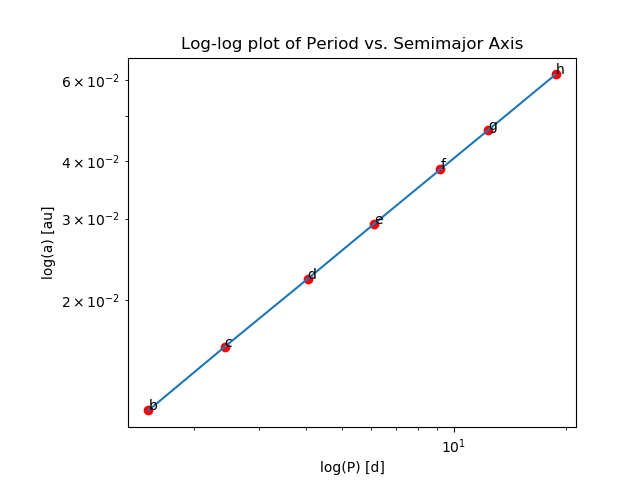
\includegraphics[width=0.75\textwidth]{prob5-a.png}
\begin{tikzpicture}
    \begin{axis}[
        title=Log-log Plot of Orbital Period vs. Semimajor Axis,
        xmode=log,
        ymode=log,
        xlabel = {\(\log(P) [\si{\day}]\)},
        ylabel = {\(\log(a) [\si{\astronomicalunit}]\)},
        log basis x = {10},
        log basis y = {10}
    ]
    \addplot table[
        only marks,
        x=p, y=a,
        col sep=comma,
    ] {data.csv};
    \addplot table[
        red,
        y={create col/linear regression={y=a}},
        col sep=comma,
        mark=none
    ] {data.csv};
    \end{axis}
\end{tikzpicture}
\end{center}

\subsection{}

\lstinputlisting{ps01.py}
Using the \lstinline|numpy.polyfit| function, we find that
\begin{align}
    m &= \num{0.6662913872826872} \\
    b &= \num{-2.058112526126338}
\end{align}

\subsection{}

\(m\) represents the (logarithmic) ratio between the semimajor axis and orbital period of a planet.
It could be used to verify Kepler's third law.

\subsection{}

The \(y\)-intercept can be used to determine the mass of the central star because it represents a \(\log(P) = 0 \Rightarrow P = 1\), since the star cannot orbit itself.
Finding \(a\),
\begin{equation}
    a = 10^b = \num{0.008747570954405929}
\end{equation}
Plugging in and letting \(m_1 + m_2\),
\begin{align}
    P^2 &= \frac{4 \pi^2}{G (2 m_1)}a^3 \\
    \Rightarrow m_1 &= \frac{2 \pi^2}{GP^2}a^3 = 
\end{align}

\end{document}
